\documentclass[french,11pt,twoside]{VcCours}

\newenvironment{ApplicationDirecte}{\textbf{Application directe du cours :}

}{}
\newcommand{\dx}{\text{d}x}
\newcommand{\dt}{\text{d}t}
\DeclareMathOperator{\e}{e}
\newcommand{\Sum}[2]{\sum_{#1}^{#2}}
\newcommand{\Int}[2]{\int_{#1}^{#2}}

\begin{document}

\Titre{PSI}{Promotion 2021--2022}{Mathématiques}{Chapitre 3 : Espaces vectoriels}

\tableofcontents
\separationTitre


Dans tout le chapitre, $n$, $k$ et $p$ seront des entiers naturels non nuls et $\mathbb{K}$ sera $\mathbb{R}$ ou $\mathbb{C}$.

\section{Espaces et sous-espaces vectoriels}
\subsection{Généralités}
\begin{Definition}{}
Un $\mathbb{K}$-\emph{espace vectoriel} est un ensemble $E$ muni d'une loi de composition interne $+ : E \times E \rightarrow E$ et d'une loi de composition externe $\cdot : \mathbb{K} \times E \rightarrow E$ tel que :
\begin{enumerate}
\item $(E, +)$ est un \emph{groupe commutatif} (ou \emph{abélien}).
%
% c'est-à-dire : 
%
%\begin{itemize}
%\item $\forall (a,b,c) \in E^3, \, a+(b+c) = (a+b)+c$ (\emph{associativité}).
%
%\item $\exists 0_E \in E \, \vert \, \forall a \in E, \, 0_E+a=a+e=0_E$ (\emph{existence d'un élément neutre})
%
%\item $\forall x \in E$, $\exists y \in E\, \vert \, x+y=y+x=0$ (\emph{existence d'un symétrique})
%
%\item $\forall (a,b) \in E^2, a+b=b+a$ (\emph{commutativité}).
%\end{itemize}
\item

\begin{itemize}
\item $\forall (\lambda, \mu) \in \mathbb{K}^2$, $\forall a \in E$, $(\lambda+\mu) \cdot a = \lambda \cdot a + \mu \cdot a$.
\item $\forall \lambda \in \mathbb{K}$, $\forall (a,b) \in E^2$, $\lambda \cdot (a+b) = \lambda \cdot a + \lambda \cdot b$.
\end{itemize}
\item $\forall (\lambda, \mu) \in \mathbb{K}^2, \, \forall a \in E, \, \lambda \cdot (\mu \cdot a) = (\lambda \mu) \cdot a$ (\emph{associativité mixte})
\item $\forall a \in E$, $1 \cdot a = a$.
\end{enumerate}
\end{Definition}

\begin{Remarques}{}
\begin{itemize}
\item Les éléments de $E$ sont appelés \emph{vecteurs} et les éléments de $\mathbb{K}$ les \emph{scalaires}.
\item Le \emph{symétrique} d'un vecteur $x$ de $E$ est unique. 
\item Si pour trois vecteurs $x$, $y$, $z$ de $E$, on a $x+y=x+z$ alors $y=z$. 
\item Le vecteur nul $0_E$ est unique. En effet, si un vecteur $x$ de $E$ vérifie la même propriété que $0_E$ alors :

\vspace{1.5cm}
\end{itemize}
\end{Remarques}{}

\begin{Proposition}{}
Soit $E$ un $\mathbb{K}$-espace vectoriel.

\begin{enumerate}
\item $\forall \lambda \in E$, $\lambda \cdot 0_E= 0_E$.
\item $\forall a \in E$, $0 \cdot a=0_E$.
\item $\forall a \in E$, $-a=(-1) \cdot a$.
\end{enumerate}
\end{Proposition}

\medskip

\begin{Exemples}
\begin{enumerate}
\item $\mathbb{K}^n$, $\mathbb{K}[X]$, $\mathcal{M}_{n,p}(\mathbb{K})$, $\mathcal{F}(X,E)$ (ensemble des fonctions définies sur un ensemble $X$ à valeurs dans un espace vectoriel $E$), $\mathcal{C}^k(I, \mathbb{K})$ sont des $\mathbb{K}$-espaces vectoriels.
\item $\mathbb{C}$ est un $\mathbb{R}-$espace vectoriel.
\end{enumerate}
\end{Exemples}

\medskip

\begin{Definition}{} Soient $E$ un $\mathbb{K}$-espace vectoriel et $(e_1, \ldots, e_p)$ une famille de vecteurs de $E$.

Un vecteur $x$ de $E$ est une \emph{combinaison linéaire} de $(e_1, \ldots, e_p)$ si 

{il existe $(\lambda_1, \ldots, \lambda_p) \in \mathbb{K}^p$ tel que :}
$$ {x = \sum_{k=1}^p \lambda_k e_k = \lambda_1 e_1 + \lambda_2 e_2 + \cdots + \lambda_p e_p }$$
\end{Definition}


\begin{Exemples}
\begin{enumerate}
\item Tout élément $(x,y)$ de $\mathbb{K}^2$ est combinaison linéaire de $e_1=(1,0)$ et $e_2=(0,1)$ :

{$(x,y) = x(1,0)+ y(0,1)= xe_1 + y e_2$}
\item Dans $\mathcal{F}(\mathbb{R},\mathbb{R})$, La fonction $x \mapsto \cos(2x)$ est combinaison linéaire de la fonction constante égale à $1$ et de $x \mapsto \sin^2(x)$ :
$$ \forall x \in \mathbb{R}, \, \cos(2x) = 1 - 2 \sin^2(x)$$
Remarquons que dans cet espace vectoriel, $f=g$ signifie : $\forall x \in \mathbb{R}$, $f(x)=g(x)$.
\end{enumerate}
\end{Exemples}



\begin{Definition}{} Soit $E$ un $\mathbb{K}$-espace vectoriel. Un \emph{sous-espace vectoriel} de $E$ est un sous-ensemble $F$ de $E$ qui, muni  des lois de composition $+$ et $\cdot$ de $E$, est un $\mathbb{K}$-espace vectoriel.
\end{Definition}

\begin{Proposition}{Méthode des trois points}
Soit $E$ un $\mathbb{K}$-espace vectoriel. $F$ est un sous-espace vectoriel de $E$ si et seulement si :
\begin{enumerate}
\item {$F \subset E$.}
\item {$0_{E} \in F$.}
\item {$\forall \lambda \in \mathbb{K}$, $\forall (x,y) \in F^2$, $\lambda x+y \in F$.}
\end{enumerate}
\end{Proposition}

\begin{Remarque}{}
$F$ est un sous-espace vectoriel de $E$ si et seulement si c'est un sous-ensemble de $E$ non vide et stable par combinaison linéaire.
\end{Remarque}

\begin{Exemples}
\begin{enumerate}
\item $\lbrace 0_E \rbrace$ et $E$ sont des sous-espaces vectoriels de $E$.
\item Soit $n \in \mathbb{N}$. Alors $\mathbb{K}_n[X]$ est un sous-espace vectoriel de $\mathbb{K}[X]$. En effet :
\begin{itemize}
\item $\mathbb{K}_n[X] \subset \mathbb{K}[X]$.
\item Le polynôme nul appartient à $\mathbb{K}_n[X]$.
\item $\forall \lambda \in \mathbb{K}$, $\forall (P,Q) \in \mathbb{K}_n[X]^2$,
$$ \textrm{deg}(\lambda P+ Q) \leq \max (\textrm{deg}(\lambda P), \textrm{deg}(Q)) \leq n$$
donc $\lambda P + Q \in \mathbb{K}_n[X]$.
\end{itemize}
\end{enumerate}
\end{Exemples}

\begin{ApplicationDirecte} Montrer que l'ensemble des matrices symétriques de $\mathcal{M}_n(\mathbb{R})$ est un sous-espace vectoriel de $\mathcal{M}_n(\mathbb{R})$. \end{ApplicationDirecte}

\begin{Proposition}{}
Soient $E$ un $\mathbb{K}$-espace vectoriel, $I$ un ensemble et $(E_i)_{i \in I}$ une famille de sous-espaces vectoriels de $E$. Alors $\bigcap_{i \in I} E_i$ est un sous-espace vectoriel de $E$.
\end{Proposition}

\begin{Demonstration}{}
On vérifie les trois points :
\begin{itemize}
\item $\bigcap_{i \in I} E_i \subset E$.
\item Pour tout $i \in I$, $O_E \in E_i$ (car $E_i$ est un sous-espace vectoriel de $E$) et donc $O_E \in \bigcap_{i \in I} E_i \subset E$.
\item Soient $\lambda \in \mathbb{K}$ et $(x,y) \in \left(\bigcap_{i \in I} E_i \right)^2$. Pour tout $i \in I$, $x$ et $y$ appartiennent à $E_i$ donc $\lambda x+y$ appartient aussi à $E_i$ (car $E_i$ est un sous-espace vectoriel de $E$) et donc $\lambda x+y$ appartient à $\bigcap_{i \in I} E_i \subset E$.
\end{itemize}
\end{Demonstration}

\begin{TheoremeDefinition}{}
Soient $E$ un $\mathbb{K}$-espace vectoriel, $n \in \mathbb{N}^*$ et $\mathcal{F}=(e_1, e_2, \ldots, e_n)$ une famille de vecteurs de $E$. On appelle \emph{espace vectoriel engendré} par $\mathcal{F}$, et on note $\Vect(\mathcal{F})$ ou $\Vect(e_1, e_2, \ldots, e_n)$, l'ensemble des combinaisons linéaires de $e_1, e_2, \ldots e_n$. Autrement dit :
$$ \Vect(\mathcal{F}) = \left\lbrace \sum_{k=1}^n \lambda_k e_k \, \big{\vert} \,  (\lambda_1, \lambda_2, \ldots, \lambda_n) \in \mathbb{K}^n \right\rbrace$$
L'espace vectoriel engendré par $\mathcal{F}$ est un sous-espace vectoriel de $E$.
\end{TheoremeDefinition}

\begin{Demonstration}{}
On vérifie les trois points :
\begin{itemize}
\item $\Vect(\mathcal{F}) \subset E$.
\item $0 e_1 + 0 e_2 + \cdots 0 e_n = 0_E$ et ainsi $0_E \in \Vect(\mathcal{F})$.
\item Soient $\lambda \in \mathbb{K}$ et $(x,y) \in \Vect(\mathcal{F})$. Par définition, il existe $(\lambda_1, \lambda_2, \ldots, \lambda_n) \in \mathbb{K}^n$ et $(\mu_1, \mu_2, \ldots, \mu_n) \in \mathbb{K}^n$ tel que :
$$ x=\sum_{k=1}^n \lambda_k e_k \quad \hbox{ et } \quad y=\sum_{k=1}^n \mu_k e_k$$
et ainsi :
$$ x+ \lambda y = \sum_{k=1}^n (\lambda_k+ \lambda \mu_k) e_k \in \Vect(\mathcal{F})$$
\end{itemize}
\end{Demonstration}

\begin{Remarque}{} On peut montrer que $\Vect(\mathcal{F})$ est en fait l'intersection de tous les espaces vectoriels de $E$ contenant $e_1, e_2, \ldots e_n$. C'est le plus petit sous-espace vectoriel (au sens de l'inclusion) contenant ces vecteurs.
\end{Remarque}

\medskip

\begin{ApplicationDirecte} Montrer que $\lbrace (3a+b,a-b,b+2c) \, \vert \, (a,b,c) \in \mathbb{R}^3 \rbrace$ est un sous-espace vectoriel engendré de $\mathbb{R}^3$.
\end{ApplicationDirecte}

\begin{Exemple} Soit $F = \lbrace (x,y,z) \in \mathbb{R}^3 \,  \vert \, x+y+z= 0 \rbrace.$ 

Pour tout $(x,y,z) \in \mathbb{R}^3$, on a :
$$ (x,y,z) \in F \Longleftrightarrow x=-y-z \Longleftrightarrow (x,y,z) = (-y-z,y,z) \Longleftrightarrow (x,y,z) = y(-1,1,0)+z(-1,0,1)$$
et ainsi $F = \Vect((-1,1,0), (-1,0,1))$.
\end{Exemple}

\begin{ApplicationDirecte} Montrer que $\lbrace (x,y,z)  \in \mathbb{R}^3 \, \vert \, x+y+z=0 \hbox{ et } x+2y=0\rbrace$ est un sous-espace vectoriel engendré de $\mathbb{R}^3$.
\end{ApplicationDirecte}

\subsection{Produit de sous-espaces vectoriels}

Soient $E$ un $\mathbb{K}$-espace vectoriel et $E_1$, $E_2$, $\ldots, E_p$ des sous-espaces vectoriels de $E$. Rappelons que le produit cartésien de ces sous-espaces est défini par :
$$ E_1 \times E_2 \times \cdots \times E_p = \left\lbrace (x_1, x_2, \ldots, x_p) \, \vert \, \forall i \in \iii{1}{p}, \, x_i \in E_i \right\rbrace$$

On munit le produit cartésien de deux lois de compositions :

\begin{itemize}
\item Une loi de composition \emph{interne} : $\forall (x_1, x_2, \ldots, x_p), (y_1, y_2, \ldots, y_p) \in E_1 \times E_2 \times \cdots \times E_p$,
$$ (x_1, x_2, \ldots, x_p) + (y_1, y_2, \ldots, y_p) = (x_1+y_1, \ldots, x_p + y_p)$$
\item Une loi de composition \emph{externe} : $\forall \lambda \in \mathbb{K}$, $\forall (x_1, x_2, \ldots, x_p) \in E_1 \times E_2 \times \cdots \times E_p$,
$$ \lambda \cdot (x_1, x_2, \ldots, x_p) = (\lambda x_1, \lambda x_2, \ldots, \lambda x_p)$$
\end{itemize}

\begin{Proposition}{}
Avec les lois de composition définies précédemment, $E_1 \times E_2 \times \cdots \times E_p$ est un $\mathbb{K}$-espace vectoriel.
\end{Proposition}







\subsection{Somme de sous-espaces vectoriels}

\begin{TheoremeDefinition}{}
Soient $E$ un $\mathbb{K}$-espace vectoriel et $E_1$, $E_2$, $\ldots, E_p$ des sous-espaces vectoriels de $E$. On définit la \emph{somme} de ces sous-espaces par :
$$ \sum_{k=1}^p E_k = E_1 + E_2 + \ldots + E_p = {\left\lbrace \sum_{k=1}^p x_k \, \big{\vert} \, (x_1, x_2, \ldots, x_p) \in E_1 \times E_2 \times \cdots E_p \right\rbrace}$$
La somme de ces sous-espaces vectoriels est un sous-espace vectoriel de $E$.
\end{TheoremeDefinition}

\begin{Demonstration}{}
On vérifie les trois points :
\begin{itemize}
\item $\Sum{k=1}{p} E_k \subset E$.
\item $0_E = \Sum{k=1}{p} 0_E$ et pour tout $k \in \iii{1}{p}$, $0_E \in E_k$ (car $E_k$ est un sous-espace vectoriel de $E$) donc $O_E \in \Sum{k=1}{p} E_k$.
\item Soient $\lambda \in \mathbb{K}$ et $(x,y) \in \left(\Sum{k=1}{p} E_k\right)^2$. Par définition, il existe $(x_1, x_2, \ldots, x_p) \in E_1 \times E_2 \times \cdots E_p$ et $(y_1, y_2, \ldots, y_p) \in E_1 \times E_2 \times \cdots E_p$ tels que :
$$ x = \sum_{k=1}^p x_k \quad \hbox{ et } y = \sum_{k=1}^p y_k $$
Ainsi :
$$ x+ \lambda y =  \sum_{k=1}^p x_k+ \lambda y_k $$
Or pour tout $k \in \iii{1}{p}$, $x_k+ \lambda y_k  \in E_k$ (car $E_k$ est un sous-espace vectoriel de $E$) donc $x+ \lambda y \in \Sum{k=1}{p} E_k$.
\end{itemize}



\end{Demonstration}

\begin{Exemple} $\mathbb{K}_n[X] = \Sum{k=0}{n} \Vect(X^k)$.
\end{Exemple}

\begin{Remarques}{}
\begin{itemize} 
\item On peut montrer que $\Sum{k=1}{p} E_k$ est le plus petit sous-espace vectoriel (au sens de l'inclusion) contenant les espaces $E_1$, $\ldots$, $E_p$. 
\item Si $F$ et $G$ sont des sous-espaces vectoriels de $E$, $F+G = \Vect(F \cup G) = \lbrace f+g \, \vert \, (f,g) \in F \times G\rbrace$.
\end{itemize}
\end{Remarques}{}

\begin{Definition}{} 
Soient $E$ un $\mathbb{K}$-espace vectoriel et $E_1$, $E_2$, $\ldots, E_p$ des sous-espaces vectoriels de $E$. On dit que la somme $\Sum{k=1}{p} E_k$ est \emph{directe} si :

pour tout $(x_1, x_2, \ldots, x_p) \in E_1 \times E_2 \times \cdots \times E_p$, on a :
$$ \sum_{k=1}^p x_k =0_E \Longrightarrow \forall k \in \iii{1}{p}, \, x_k = 0_E$$
Dans ce cas, la somme se note $\bigoplus_{k=1}^p E_k = E_1 \oplus \cdots \oplus E_p$.
\end{Definition}

\begin{Proposition}{}
Soient $E$ un $\mathbb{K}$-espace vectoriel et $E_1$, $E_2$, $\ldots, E_p$ des sous-espaces vectoriels de $E$. Les assertions suivantes sont équivalentes :
\begin{enumerate}
\item La somme $\Sum{k=1}{p} E_k$ est directe.
\item Tout élément $x$ de $\Sum{k=1}{p} E_k$ se décompose de manière \emph{unique} sous la forme $x = x_1 + x_2 + \ldots + x_p$ où pour tout $k \in \iii{1}{p}$, $x_k \in E_k$.
\end{enumerate}
\end{Proposition}

\begin{Demonstration}{} On raisonne par double implications.



$\rhd$ Supposons que la somme soit directe et fixons $x$ un élément de la somme. Supposons que $x$ admette deux décompositions : il existe $(x_1, x_2, \ldots, x_p)$ et $(y_1, y_2, \ldots, y_p)$ deux éléments de $E_1 \times E_2 \times \cdots \times E_p$ tels que :
$$ x = \sum_{k=1}^p x_k  = \sum_{k=1}^p y_k$$
et ainsi :
$$ \sum_{k=1}^p x_k -y_k = 0_E $$
Or, pour tout $k \in \iii{1}{p}$, $x_k-y_k \in E_k$ (car $E_k$ est un sous-espace vectoriel de $E$). Sachant que ma somme est directe, on a donc pour $k \in \iii{1}{p}$, $x_k-y_k = 0_E$ ou encore $x_k=y_k$. On obtient ainsi l'unicité de la décomposition.

\medskip

$\rhd$ Supposons que la décomposition de tout élément de $\Sum{k=1}{p} E_k$ soit unique. Montrons que la somme est directe : soit $(x_1, x_2, \ldots, x_p) \in E_1 \times E_2 \times \cdots \times E_p$ tel que :
$$ \sum_{k=1}^p x_k = 0_E $$
On a alors :
$$ \sum_{k=1}^p x_k = \sum_{k=1}^p 0_E$$
Sachant que le vecteur appartient à tous les espaces vectoriels $E_k$ ($1 \leq k \leq p$), on a par unicité de la décomposition que pour tout $k \in \iii{1}{p}$, $x_k=0_E$. Ainsi, la somme est directe.
\end{Demonstration}
 
 Dans le cas de deux sous-espaces vectoriels, on a un critère rapide pour démontrer qu'une somme est directe.
 
 \begin{Proposition}{}\label{SommeDir2}
 Soient $E$ un $\mathbb{K}$-espace vectoriel et $E_1$, $E_2$ deux sous-espaces vectoriels de $E$. Alors :
 $$ E_1 + E_2 \hbox{ est directe si et seulement si }{ E_1 \cap E_2 = \lbrace 0_E \rbrace} $$
 \end{Proposition}
 
 \begin{Demonstration}{} On raisonne par double implications.

$\rhd$ Supposons que $E_1 + E_2$ est directe. Il est clair que  $\lbrace 0_E \rbrace \subset E_1 \cap E_2$ car $E_1$ et $E_2$ sont deux sous-espaces vectoriels de $E$. Soit $x \in E_1 \cap E_2$. Alors $-x \in E_1 \cap E_2$ car $E_1$ et $E_2$ sont deux sous-espaces vectoriels de $E$ et ainsi $x+(-x) = 0_E$ avec $x \in E_1$ et $-x \in E_2$. La somme étant directe, on a $x=-x=0_E$.

\medskip

$\rhd$  Supposons que $E_1 \cap E_2 = \lbrace 0_E \rbrace$ et montrons que la somme est directe. Soit $(x_1,x_2) \in E_1 \times E_2$ tel que $x_1+x_2 = 0$. Alors $x_1=-x_2 \in E_1 \cap E_2$ car $E_2$ est un sous-espace vectoriel de $E$. Or l'intersection est réduite au vecteur nul donc $x_1=-x_2 = 0_E$ et la somme est donc directe.
\end{Demonstration}

\begin{Remarque}{} Le critère précédent ne se généralise pas dans le cas $n$ sous-espaces vectoriels avec $n \geq 3$. Par exemple :
$$ \Vect((1,0)) + \Vect((0,1)) + \Vect((1,1)) $$
n'est pas directe car $(1,1)= (1,0) + (0,1)$ (on a donc deux décompositions différentes pour le même vecteur) mais pourtant l'intersection de deux sous-espaces vectoriels parmi les trois précédents est toujours réduite au vecteur nul.
\end{Remarque}


\begin{Definition}{}
Soient $E$ un $\mathbb{K}$-espace vectoriel et $E_1$, $E_2$, $\ldots, E_p$ des sous-espaces vectoriels de $E$.  On dit que les espaces $E_1$, $E_2$, $\ldots, E_p$ sont \emph{supplémentaires} si $E = E_1 \oplus E_2 \oplus \cdots \oplus E_p$ ou autrement dit, si :
$$ \forall x \in E, \, \exists ! (x_1, x_2, \ldots, x_p) \in E_1 \times E_2 \times \cdots \times E_p \, \vert \, x= x_1 + x_2 + \ldots + x_p$$
\vspace{1cm}
\end{Definition}
\medskip

\begin{Exemple} Soient $F = \left\lbrace f \in \mathcal{C}([-1,1], \mathbb{R}) \, \big{\vert} \, \int_{ - 1}^{1} f(t) \dt = 0\right\rbrace$ et $G = \left\lbrace  f \in \mathcal{C}([-1,1], \mathbb{R})\, \vert \, f \, \hbox{ est constante} \right\rbrace$
Montrons que $F$ et $G$ sont des sous-espaces vectoriels supplémentaires de $\mathcal{C}([-1,1], \mathbb{R})$.
\begin{enumerate}
\item $F$ et $G$ sont des sous-espaces vectoriels de $\mathcal{C}([-1,1], \mathbb{R})$.
\item Raisonnons par analyse-synthèse.

$\rhd$ \emph{Analyse :} soit $f \in \mathcal{C}([-1,1], \mathbb{R})$. Supposons l'existence de $(f_1,f_2) \in F \times G$, tel que $f=f_1+f_2$. La fonction $f_2$ est constante (disons de constante égale à $c \in \mathbb{R}$). On a alors par linéarité de l'intégrale :
$$ \int_{-1}^{1} f(x) \dx = \int_{-1}^{1} f_1(x) \dx + \int_{-1}^{1} c \dx = 2c $$
car $f_1 \in F$. Ainsi $c = \dfrac{1}{2} \Int{-1}{1} f(x) \dx$. On a donc pour tout $x \in [-1,1]$, $f_2(x) = \Int{-1}{1} f(x) \dx$ et 
$$ f_1(x) = f(x)-f_2(x) = f(x) - \dfrac{1}{2} \Int{-1}{1} f(x) \dx$$

\medskip

$\rhd$ \emph{Synthèse :} Soit $f \in \mathcal{C}([-1,1], \mathbb{R})$. Posons pour tout $x \in [-1,1]$, $f_2(x) = \dfrac{1}{2}\Int{-1}{1} f(x) \dx$ et 
$$ f_1(x) = f(x)-f_2(x) = f(x) - \dfrac{1}{2} \Int{-1}{1} f(x) \dx$$
On a bien $f=f_1+f_2$, $f_2$ est constante donc $f_2 \in G$ et par linéarité de l'intégrale,
$$ \int_{-1}^{1} f_1(x) \dx = \int_{-1}^{1} f(x) \dx - \Int{-1}{1} f_2(x) \dx = \int_{-1}^{1} f(x) \dx - 2 \times \dfrac{1}{2} \int_{-1}^{1} f(x) \dx = 0$$
donc $f_1 \in F$. Ainsi $f$ est somme d'un élément de $F$ et d'un élément de $G$ et l'unicité de la décomposition provient de l'analyse.

\medskip

$\rhd$ On a donc $\mathcal{C}([-1,1], \mathbb{R}) = F \bigoplus G$.
\end{enumerate}

\end{Exemple}
%
%\begin{ApplicationDirecte} Prouver le résultat de la question 1. de l'exemple précédent.
%\end{ApplicationDirecte}

\begin{ApplicationDirecte}\label{Exo}  En raisonnant par analyse-synthèse, montrer que les espaces 
$$ F = \lbrace (x_1, \ldots, x_n) \, \vert \, x_1 + \cdots + x_n = 0 \rbrace \; \hbox{ et } \; G= \Vect((1, \ldots, 1)) $$
sont supplémentaires dans $\mathbb{R}^n$.
\end{ApplicationDirecte}

Dans le cas de deux espaces vectoriels, on a un critère plus rapide pour montrer que deux sous-espaces vectoriels sont supplémentaires.

 \begin{Proposition}{}
 Soient $F$ un $\mathbb{K}$-espace vectoriel et $E_1$, $E_2$ deux sous-espaces vectoriels de $E$. Alors :
 $$ E_1 \hbox{ et } E_2 \hbox{ sont supplémentaires si et seulement si } \left\lbrace\begin{array}{l}
 E=E_1+ E_2 \\
 E_1 \cap E_2 = \lbrace 0_E \rbrace
 \end{array}\right.$$
 \end{Proposition}
 
 \begin{Demonstration}{}
 Conséquence de la proposition \ref{SommeDir2}.
 \end{Demonstration}

 
 \section{Familles libres, génératrices, bases}
 
 \begin{Definition}{}
Soient $E$ un $\mathbb{K}$-espace vectoriel et $\mathcal{F} = (e_1, e_2, \ldots, e_p)$ une famille de vecteurs de $E$.

\begin{itemize}
\item On dit que $\mathcal{F}$ est \emph{libre} si  :

pour pour tout $(\lambda_1, \lambda_2, \ldots, \lambda_p) \in \mathbb{K}^p$,
$$ \sum_{k=1}^p \lambda_k e_k = 0_E \Rightarrow \forall k \in \iii{1}{p}, \, \lambda_k = 0$$

On dit que les vecteurs $e_1$, $e_2$, $\ldots$, $e_p$ sont \emph{linéairement indépendants}.
\item On dit que $\mathcal{F}$ est \emph{liée} si elle n'est pas libre ce qui équivaut à l'existence d'un $p$-uplet \newline $(\lambda_1, \lambda_2, \ldots, \lambda_p) \in \mathbb{K}^p \setminus \lbrace (0,0, \ldots,0) \rbrace$ tel que :
$$ \sum_{k=1}^p \lambda_k e_k = 0_E$$
On dit que les vecteurs $e_1$, $e_2$, $\ldots$, $e_p$ sont \emph{linéairement dépendants}.
\item On dit que $\mathcal{F}$ est \emph{génératrice} de $E$ si tout élément de $E$ s'écrit comme une combinaison linéaire d'éléments de $\mathcal{F}$, autrement dit si :
$$ \forall x \in E, \, \exists (\lambda_1, \lambda_2, \ldots, \lambda_p) \in \mathbb{K}^p \, \big{\vert} \, x=\sum_{k=1}^p \lambda_k e_k$$


ou de manière équivalente si $E = \Vect(\mathcal{F})$.

On dit que les vecteurs $e_1$, $e_2$, $\ldots$, $e_p$ \emph{engendrent} $E$.
\item On dit que $\mathcal{F}$ est une \emph{base} de $E$ si elle est à la fois libre et génératrice.
\end{itemize}
\end{Definition}

\begin{Remarque}{}
	\warning{} Il faut se méfier de la négation d'être une famille libre : 
	une famille est liée si il existe des scalaires \emph{non tous nuls} 
	(et non pas tous non nuls) donnant une combinaison linéaire nulle.
\end{Remarque}

\medskip

\begin{Definition}{} Deux vecteurs $x$ et $y$ d'un $\mathbb{K}$-espace vectoriel $E$ sont dit \emph{colinéaires} si il existe $\alpha \in \mathbb{K}$ tel que $y= \alpha x$ ou tel que $x= \alpha y$.
\end{Definition}

\begin{Proposition}{}
Soient $E$ un $\mathbb{K}$-espace vectoriel et $(x,y)$ un couple de vecteurs de $E$.

\begin{enumerate}
\item $(x)$ est une famille libre si et seulement si $x \neq 0_E$.
\item $(x,y)$ est une famille libre si et seulement $x$ et $y$ ne sont pas colinéaires.
\end{enumerate}
\end{Proposition}
%
%\begin{Demonstration}{}
%\vspace{7cm}
%%
%%\begin{enumerate}
%%\item Si $x \neq 0_E$ et si $\lambda \in \mathbb{K}$ alors $\lambda x = 0_E$ implique $\lambda = 0$ et donc $(x)$ est libre. Si $x=0_E$ alors par exemple $2x=0_E$ et pourtant $2 \neq 0$ donc $(x)$ n'est pas libre.
%%\item Supposons que $(x,y)$ est une famille libre. Par l'absurde, si $x$ et $y$ sont colinéaires, il existe $\alpha \in \mathbb{K}$ tel que $y = \alpha x$ ou $x= \alpha y$ ce qui implique que $y- \alpha x= 0_E$ ou $x-\alpha y = 0_E$ et donc par liberté $1= 0$ ce qui est absurde.
%%
%%\medskip
%%
%%Si $(x,y)$ est liée alors existe $\lambda_1$, $\lambda_2$ non tous les deux nuls tel que $\lambda_1 x + \lambda_2 y = 0_E$. Le résultat est alors clair en remarquant qu'un des deux réels $\lambda_1$ et $\lambda_2$ est non nul.
%%\end{enumerate}
%\end{Demonstration}

\begin{Exemple} Étudions dans $\mathbb{R}^3$ la liberté de la famille $((1,2,1), (1,-1,1), (1,1,0))$.

\vspace*{8cm}
\end{Exemple}

\begin{ApplicationDirecte} Étudier dans $\mathbb{R}[X]$ la liberté de la famille ($(1-X)^2,X(1-X),X^2)$.
\end{ApplicationDirecte}
\begin{Exemple} Soient $n \in \mathbb{N}^*$ et $(P_1, P_2, \ldots, P_n)$ une famille de $\mathbb{R}[X]$. On suppose que :
$$ 0 \leq \textrm{deg}(P_1) < \textrm{deg}(P_2) < \cdots < \textrm{deg}(P_n)$$
On dit que la famille est \emph{échelonnée en degré} (et qu'elle ne contient pas le polynôme nul). Montrons que cette famille est libre.

\medskip

Soit $(\lambda_1, \lambda_2, \ldots, \lambda_n) \in \mathbb{K}^n$ tel que :
$$ \sum_{k=1}^n \lambda_k P_k = 0_{\mathbb{K}[X]}$$
Supposons par l'absurde que $(\lambda_1, \lambda_2, \ldots, \lambda_n)$ n'est pas nul. On pose alors :
$$ j = \max \lbrace k \in \iii{1}{n}, \, \vert \, \lambda_k \neq 0 \rbrace$$
Notons que $j$ existe car c'est le maximum d'un ensemble fini non vide. On a alors :
$$ \sum_{k=1}^j \lambda_k P_k = O_{\mathbb{K}[X]}$$
ou encore :
$$ \sum_{k=1}^{j-1} \lambda_k P_k = - \lambda_j P_j $$
Par somme, le polynôme
$$\sum_{k=1}^{j-1} \lambda_k P_k $$
est au plus de degré $\textrm{deg}(P_{j-1})$ qui est strictement plus petit que $\textrm{deg}(P_{j})$. Nécessairement, on a donc $\lambda_j = 0$ ce qui est absurde au vu de la définition de $j$.

Ainsi $\lambda_1 = \lambda_2 = \ldots = \lambda_n = 0$ et la famille est donc libre.
\end{Exemple}

\begin{TheoremeDefinition}{} 
Soient $E$ un $\mathbb{K}$-espace vectoriel et $\mathcal{F} = (e_1, e_2, \ldots, e_p)$ une famille de vecteurs de $E$. Alors $\mathcal{F}$ est une base de $E$ si et seulement si :
$$ \forall x \in E, \, \exists  ! (\lambda_1, \lambda_2, \ldots, \lambda_p) \in \mathbb{K}^p \, \big{\vert} \, x = \sum_{k=1}^p \lambda_k e_k$$
Le $p$-uplet $(\lambda_1, \lambda_2, \ldots, \lambda_p)$ est appelé \emph{coordonnées} (ou \emph{composantes}) de $x$ dans la base $\mathcal{F}$.
\end{TheoremeDefinition}

\section{Espaces vectoriels de dimension finie}
 \subsection{Définition et premières propriétés}
 \begin{Definition}{} On dit qu'un espace vectoriel est de \emph{dimension finie} si il admet une famille génératrice finie. Sinon, il est dit de \emph{dimension infinie}.
 \end{Definition}
 
% \begin{Theoreme}{}\label{BaseDimFi}
% Tout espace vectoriel, non réduit au vecteur nul et de dimension finie admet une base.
% \end{Theoreme}
 
 \begin{Theoreme}{Base incomplète}\label{BaseInc}
 Soit $E$ un espace vectoriel de dimension finie. Tout famille libre d'éléments de $E$ peut être complétée en une base de $E$. Pour compléter une telle famille, il suffit de choisir dans une famille génératrice de $E$ des éléments n'appartenant pas à la famille libre.
 
 \medskip
 
En particulier, tout espace vectoriel, non réduit au vecteur nul et de dimension finie admet une base.
 \end{Theoreme}
% 
% \begin{Remarque}{} L'idée de la preuve du théorème est de montrer que toute sous-famille libre de la famille génératrice de l'espace peut être complété en une base de $E$ à l'aide d'éléments de la famille génératrice.
% \end{Remarque}
% 

 \begin{Theoreme}{} Toutes les bases d'un $\mathbb{K}$-espace vectoriel $E$ non réduit au vecteur nul de dimension finie ont le même cardinal. Ce nombre est appelé \emph{dimension} de $E$ et on le note $\textrm{dim}_{\mathbb{K}}(E)$ ou $\textrm{dim}(E)$ (si il n'y a pas d'ambiguïté sur le corps de base). Par convention, si $E$ est réduit au vecteur nul, sa dimension est nulle.
 \end{Theoreme}
 

 
 Donnons maintenant des exemples (usuels) en donnant à chaque fois la \emph{base canonique} (c'est-à-dire la base la plus classique).
 
 \medskip
 
 \begin{Exemples}
\begin{enumerate}
 \item Base canonique de $\mathbb{K}^n$ : 
 
 $e_1 = (1, 0 , \ldots , 0)$, $\ldots$, $e_n = (0, 0, \ldots, 1)$. On a ainsi $\textrm{dim}(\mathbb{K}^n)=n$.
 \item Base canonique de $\mathcal{M}_{n,p}(\mathbb{K})$ : $(E_{i,j})_{1 \leq i \leq n, 1 \leq j \leq p}$ où $E_{i,j}$ est la matrice de taille $n \times p$ dont tous les coefficients son nuls exceptés celui de la $i$-ième ligne et $j$-ième colonne qui vaut $1$. On a ainsi $\textrm{dim}(\mathcal{M}_{n,p}(\mathbb{K}))=n \times p$.
 \item Base canonique de $\mathbb{K}_n[X]$ : 
 
 $(1,X,X^2, \ldots, X^n)$. On a ainsi $\textrm{dim}(\mathbb{K}_n[X])=n+1$.
 \item $\mathbb{C}$ est $\mathbb{C}-$espace vectoriel, $(1)$ est une base et $\textrm{dim}_{\mathbb{C}}(\mathbb{C})=1$ alors que $\mathbb{C}$ est $\mathbb{R}-$espace vectoriel, $(1,i)$ est une base et $\textrm{dim}_{\mathbb{R}}(\mathbb{C})=2$.
 \end{enumerate}
\end{Exemples}
 
 \begin{Proposition}{}
 Soient $E$ un $\mathbb{K}$-espace vectoriel de dimension finie $n \geq 1$. Si $\mathcal{F}$ est une famille de $n$ vecteurs de $E$ alors on a les équivalences suivantes : 
$$ {\mathcal{F} \hbox{ est une base de E} \Longleftrightarrow \mathcal{F} \hbox{ est libre } \Longleftrightarrow \mathcal{F} \hbox{ est génératrice de E }}$$
\end{Proposition}

\begin{Exemple} Soient $n \in \mathbb{N}^*$ et $(P_0,P_1, \ldots, P_n)$ une famille de polynômes de $\mathbb{K}[X]$ tels que pour tout $k \in \iii{0}{n}$, $\textrm{deg}(P) = k$. Alors $(P_0,P_1, \ldots, P_n)$ est une base de $\mathbb{K}_n[X]$.

En effet, la famille est échelonné en degrés, ne contient pas le vecteur nul et donc est libre dans $\mathbb{K}_n[X]$. Or la dimension de $\mathbb{K}_n[X]$ est $n+1$ qui est le cardinal de $\mathbb{K}_n[X]$ donc c'est une base de $\mathbb{K}_n[X]$.
\end{Exemple}

\medskip

\begin{Remarque}{} Si $E$ est un $\mathbb{K}$-espace vectoriel de dimension finie $n \geq 1$ alors toute famille libre de $E$ a un cardinal inférieur ou égal à $n$ et toute famille génératrice a un cardinal supérieur ou égal à $n$.
\end{Remarque}

\begin{ApplicationDirecte} Soient $E$ un $\mathbb{K}$-espace vectoriel de dimension 3 et $\mathcal{B} = (e_{1} ,e_{2} ,e_{3})$ une base de $E$. Posons :
  \[
  \varepsilon_{1} = e_{2} + 2e_{3} , \, \varepsilon_{2} = e_{3} - e_{1} \; \hbox{ et } \; \varepsilon_{3} = e_{1} + 2e_{2}
  \]
Montrer que $\mathcal{B}' = (\varepsilon_{1} ,\varepsilon_{2} ,\varepsilon_{3})$ est une base de $E$.
\end{ApplicationDirecte}

\medskip
\subsection{Dimension de sous-espaces vectoriels, de produits, de sommes}

\begin{Proposition}{}  Soient $E$ un $\mathbb{K}$-espace vectoriel de dimension finie et $F$ un sous-espace vectoriel de $E$. Alors :

\begin{itemize}
\item $F$ est de dimension finie et $\textrm{dim}(F) \leq \textrm{dim}(E)$.
\item De plus, si $\textrm{dim}(F) = \textrm{dim}(E)$ alors $F=E$.
\end{itemize}
\end{Proposition}

\begin{ApplicationDirecte} Montrer que, dans $\mathbb{R}^3$, $\Vect((1,1,0), (-1,2,1))= \Vect((0,3,1), (3,0,-1))$.
\end{ApplicationDirecte}

\begin{Proposition}{}
Soient $E$ un $\mathbb{K}$-espace vectoriel et $E_1$, $E_2$, $\ldots, E_p$ des sous-espaces vectoriels de $E$ de \emph{dimensions finies}. Alors $E_1 \times E_2 \times \cdots \times E_p$ est un $\mathbb{K}$-espace vectoriel de dimension finie et :
$$ \textrm{dim}(E_1 \times E_2 \times \cdots \times E_p) = \sum_{k=1}^p \textrm{dim} (E_k)$$
\end{Proposition}

\begin{Demonstration}{} On pose pour tout $k \in \iii{1}{p}$, 
	$n_k = \textrm{dim} (E_k)$ et $(e_{k,1}, \, e_{k,2}, \, \ldots, \, e_{k,n_k})$ 
	une base de $E_k$. On montre alors que la famille 
	$((e_{1,1}, 0_{E_2}, \ldots, 0_{E_p})$, $\ldots$, 
	$(e_{1,n_1}, 0_{E_2}, \ldots, 0_{E_p})$, $\ldots$, 
	$(0_{E_1},e_{2,1}, 0_{E_2}, \ldots, 0_{E_p})$, $\ldots$,
	$(0_{E_1},e_{2,n_2}, 0_{E_2}, \ldots,0_{E_p}),$
	$(0_{E_1},e_{2,n_2}, 0_{E_2}, \ldots,0_{E_p})$, $\ldots$, 
	$(0_{E_1},\ldots, 0_{E_{p-1}}, e_{p,1})$, $(0_{E_1},\ldots, 
	0_{E_{p-1}}, e_{p,n_p}))$ est une base de $E_1 \times E_2 \times \cdots \times E_p$
	ce qui donne le résultat.
\end{Demonstration}

%\begin{lem}
%Soient $E$ un espace vectoriel, $p \in \mathbb{N}^*$ tel que $p \geq 2$ et $(x_1, x_2, \ldots, x_p)$ une famille libre. Alors pour tout $i \in \iii{1}{p-1}$,
%$$ \Vect(x_1, x_2, \ldots, x_p) = \Vect(x_1, \ldots, x_i) \oplus \Vect(x_{i+1}, \ldots, x_p)$$
%\end{lem}

%\begin{Demonstration}{}
%Les inclusions 
%$$ \Vect(x_1, x_2, \ldots, x_p) \subset \Vect(x_1, \ldots, x_i) + \Vect(x_{i+1}, \ldots, x_p)$$
%et 
%$$ \Vect(x_1, \ldots, x_i) + \Vect(x_{i+1}, \ldots, x_p) \subset \Vect(x_1, x_2, \ldots, x_p) $$
%sont claires. Montrons que $\Vect(x_1, \ldots, x_i) + \Vect(x_{i+1}, \ldots, x_p)$ est directe : soit $(y,z) \in \Vect(x_1, \ldots, x_i) \times \Vect(x_{i+1}, \ldots, x_p)$ tel que $y+z = 0_E$. Par définition, il existe des scalaires $\lambda_1, \lambda_2, \ldots, \lambda_p$ tels que 
%$$y = \sum_{k=1}^i \lambda_k x_k \quad \hbox{ et } \quad z = \sum_{k=i+1}^p \lambda_k x_k $$
%et ainsi :
%$$ \sum_{k=1}^p\lambda_k x_k =  0_E $$
%Or $(x_1, x_2, \ldots, x_p)$ est libre donc pour tout $k \in \iii{1}{p}$, $\lambda_k$ et donc $y=z=0_E$ et ainsi la somme est directe.
%\end{Demonstration}

\begin{Proposition}{Fractionnement d'une base}\label{UnionBase} Soient $E$ un $\mathbb{K}$-espace vectoriel de dimension finie, $p \in \mathbb{N}^*$ avec $p \geq 2$ et $E_1$, $E_2$, $\ldots$, $E_p$ des sous-espaces vectoriels de $E$ munis de bases $\mathcal{B}_1$, $\mathcal{B}_2$, $\ldots$, $\mathcal{B}_p$. Alors :
$$ E= E_1 \oplus E_2 \oplus \cdots \oplus E_p \Longleftrightarrow  \bigcup_{k=1}^p \mathcal{B}_k \hbox{ est une base de } E$$
\end{Proposition}

\begin{Demonstration}{} On procède par double implications. On note pour tout $k \in \iii{1}{p}$, $n_k$ la dimension de $E_k$ et $(e_{k,1}, e_{k,2}, \ldots, e_{k,n_k})$ la base $\mathcal{B}_k$.

\medskip

$\rhd$ Supposons que $E= E_1 \oplus E_2 \oplus \cdots \oplus E_p$. Soit $x \in E$. Il existe alors $(x_1, x_2, \ldots, x_p) \in E_1 \times E_2 \times \cdots \times E_p$ tel que :
$$ x = \sum_{k=1}^p x_k $$
Or, pour tout $k \in \iii{1}{p}$, $x_k$ s'écrit comme une combinaison linéaire d'éléments de $\mathcal{B}_k$ (car c'est une base de $E_k$) et ainsi s'écrit comme une combinaison linéaire d'éléments de $\bigcup_{k=1}^p \mathcal{B}_k$ qui est ainsi génératrice. 

\medskip 

Montrons maintenant que $\bigcup_{k=1}^p \mathcal{B}_k$ est libre. Pour tout $k \in \iii{1}{p}$, considérons une famille de scalaire $(\lambda_{k,j})_{1 \leq j \leq n_k}$. Supposons que :
$$ \sum_{k=1}^p \sum_{i=1}^{n_i} \lambda_{k,i} e_{k,i} = 0_E$$
Or pour tout $k \in \iii{1}{p}$, $\Sum{i=1}{n_i} \lambda_{k,i} e_{k,i}$ appartient à $E_k$. La somme des $E_k$ étant directe, on a alors que pour tout $k \in \iii{1}{p}$,
$$ \sum_{i=1}^{n_i} \lambda_{k,i} e_{k,i}$$
et sachant que $\mathcal{B}_k$ est une base et en particulier une famille libre :
$$ \forall i \in \iii{1}{n_i}, \, \lambda_{k,i} = 0$$
et donc $\mathcal{B}$ est bien libre.

\medskip

$\rhd$ Supposons que $\bigcup_{k=1}^p \mathcal{B}_k$ soit une base de $E$. On a :
$$ E= E_1 + E_2 + \cdots + E_p $$
En effet : $E \subset E_1 + E_2 + \cdots + E_p$ car $\bigcup_{k=1}^p \mathcal{B}_k$ est génératrice et l'autre inclusion est claire. Montrons maintenant que la somme est directe : soit $(x_1, x_2, \ldots, x_p) \in E_1 \times E_2 \times \cdots E_p$ tel que :
\begin{equation}\label{Frac} 
\sum_{k=1}^p x_k = 0
\end{equation}
Pour tout $k \in \iii{1}{p}$, $x_k \in E_k$ et $\mathcal{B}_k$ est une base de $E_k$ donc il existe une famille de scalaires $(\lambda_{k,j})_{1 \leq j \leq n_k}$ tel que :
$$ x_k = \sum_{i=1}^{n_i} \lambda_{k,i} e_{k,i}$$
Et donc d'après (\ref{Frac}), 
$$ \sum_{k=1}^p \sum_{i=1}^{n_i} \lambda_{k,i} e_{k,i} = 0_E$$
Or $\mathcal{B}$ est une base donc tous les scalaire $\lambda_{k,i}$ sont nuls et ainsi $x_1 = x_2 = \ldots = x_p = 0_E$. La somme est donc bien directe.

\end{Demonstration}

\begin{Definition}{} Dans le cas où l'équivalence de la proposition précédente est vraie, on appelle \emph{base adaptée} à la décomposition en somme directe toute base $\mathcal{B}$ de $E$ s'écrivant sous la forme $\bigcup_{k=1}^p \mathcal{B}_k$ où $\mathcal{B}_k$ est une base de $E_k$.
\end{Definition}

\textbf{Application : fractionnement d'une base.}

Soient $E$ est un $\mathbb{K}$-espace vectoriel de dimension finie $n \in \mathbb{N}^*$ avec $n \geq 2$ et $\mathcal{B}=(e_1, e_2, \ldots, e_n)$ une base de $E$. Alors toute partition de $\mathcal{B}$ (famille de sous-ensembles disjoints de $\mathcal{B}$ dont la réunion est $\mathcal{B}$) admettant au moins deux éléments fournit une décomposition de $E$ en somme directe.

\medskip

\begin{Exemple} Soient $E$ un $\mathbb{K}$-espace vectoriel de dimension $3$ et $(e_1,e_2,e_3)$ une base de $E$. Alors par fractionnement :
$$ E = \Vect(e_1) \oplus \Vect(e_2,e_3) = \Vect(e_1,e_2) \oplus \Vect(e_3) = \Vect(e_1,e_3) \oplus \Vect(e_2) $$
\end{Exemple}

\medskip

\begin{Corollaire}{} Soit $E$ un $\mathbb{K}$-espace vectoriel de dimension finie. Si $F$ est un sous-espace vectoriel de $E$ alors $F$ admet des sous-espaces supplémentaires.
\end{Corollaire}

\begin{Demonstration}{} Distinguons deux cas.

$\rhd$ Si $F$ est réduit au vecteur nul, c'est évident ($E$ est un supplémentaire) et si $F=E$, c'est évident aussi ($\lbrace 0_E\rbrace$ est un supplémentaire).

\medskip

$\rhd$ $F$ est un sous-espace vectoriel de $E$ qui est de dimension finie et non réduit au vecteur nul donc $F$ est de dimension finie et admet donc une base, notée $\mathcal{F}$. D'après le théorème de la base incomplète, on peut déterminer une famille $\mathcal{G}$ (d'éléments n'appartenant pas à $\mathcal{F}$ et appartenant à une famille génératrice de $E$) telle que $\mathcal{F} \cup \mathcal{G}$ soit une base de $E$. Par fractionnement d'une base, $\Vect(\mathcal{G})$ est un supplémentaire de $F$ dans $E$.
\end{Demonstration}

\medskip

\begin{Remarque}{} 
	\warning{} Un supplémentaire n'est pas unique. 
	Par exemple, dans $\mathbb{R}^2$, on a :
$$ \mathbb{R}^2 = \Vect((1,0)) \oplus \Vect((0,1)) = \Vect((1,0)) \oplus \Vect((1,1))$$

\medskip

%\begin{center}
%\emph{{\large Illustration graphique}}
%\end{center}

\begin{center}
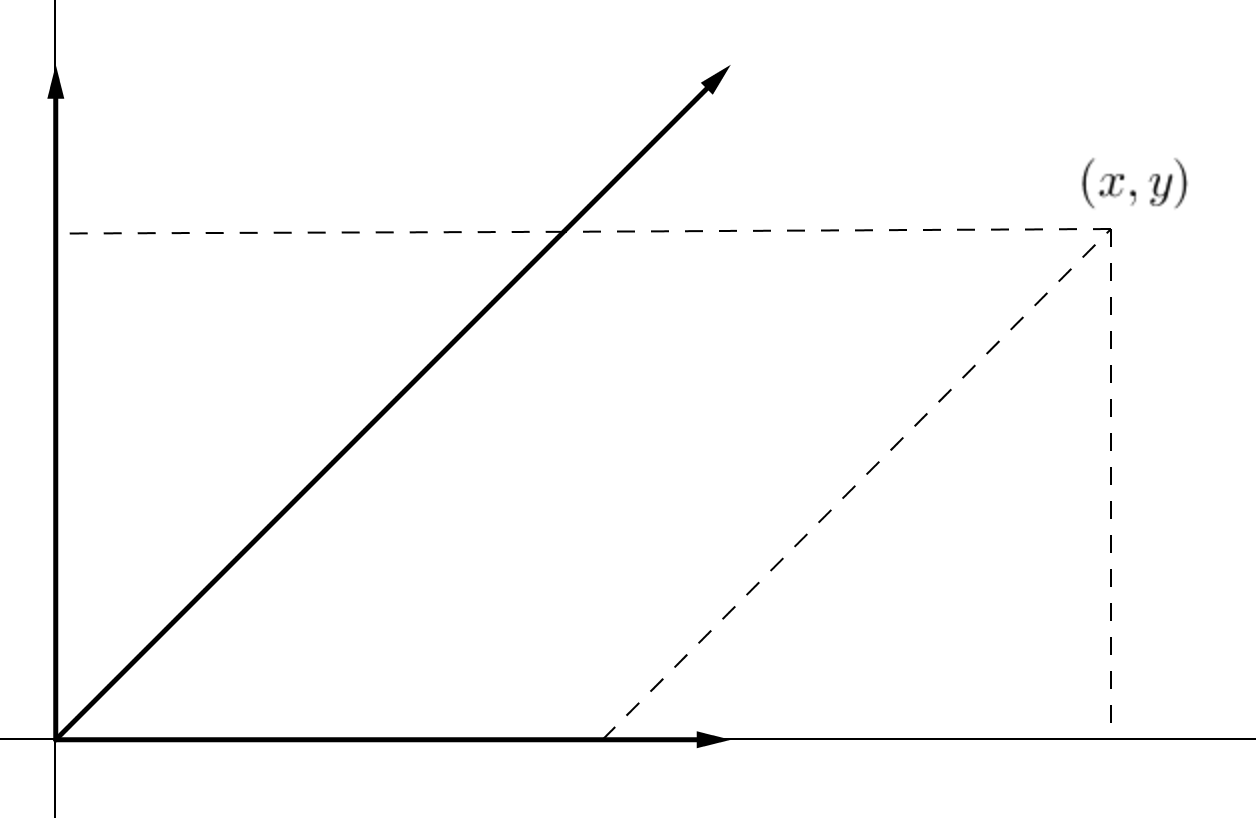
\includegraphics[scale=0.3]{Supp}
\end{center}
\end{Remarque}

\begin{Proposition}{} 
Soient $E$ un $\mathbb{K}$-espace vectoriel de dimension finie, $p \in \mathbb{N}^*$ tel que $p \geq 2$ et $(E_1, E_2, \ldots, E_p)$ des sous-espaces vectoriels de $E$. Si les espaces $E_1, E_2, \ldots, E_p$ sont en somme directe alors :
$$ \textrm{dim}(E_1 \oplus E_2 \oplus \cdots \oplus E_p) =\textrm{dim}(E_1) + \textrm{dim}(E_2) + \cdots \textrm{dim}(E_p)$$
Et en particulier si les espaces sont supplémentaires, on a :
$$ \textrm{dim}(E) = \textrm{dim}(E_1) + \textrm{dim}(E_2) + \cdots \textrm{dim}(E_p)$$
\end{Proposition}

\begin{Demonstration}{} 

D'après la proposition (\ref{UnionBase}), on sait que si la somme est directe alors $\bigcup_{k=1}^p \mathcal{B}_k \hbox{ est une base de } E_1 \oplus E_2 \oplus \cdots \oplus E_p$ et bien entendu l'union est disjointe (car la somme est directe). Ainsi :
$$ \begin{array}{ccl}
\textrm{dim}(E_1 \oplus E_2 \oplus \cdots \oplus E_p) & = & \textrm{Card} \left(\bigcup_{k=1}^p \mathcal{B}_k \right) \\
& = & \sum_{k=1}^p  \textrm{Card}(\mathcal{B}_k) \\
& = & \sum_{k=1}^p \textrm{dim}(E_k) \\
\end{array}$$
\end{Demonstration}

\begin{Corollaire}{} Soient $E$ un $\mathbb{K}$-espace vectoriel de dimension finie, $p \in \mathbb{N}^*$ tel que $p \geq 2$ et $(E_1, E_2, \ldots, E_p)$ des sous-espaces vectoriels de $E$. Si les espaces $E_1, E_2, \ldots, E_p$ sont en somme directe alors :
$$ E = E_1 \oplus E_2 \oplus \cdots \oplus E_p \Longleftrightarrow  \textrm{dim}(E) = \textrm{dim}(E_1) + \textrm{dim}(E_2) + \cdots \textrm{dim}(E_p)$$
\end{Corollaire}

%\begin{Demonstration}{} Évident.
%\end{Demonstration}

\begin{Proposition}{\emph{Formule de Grassman}} Soient $F$ et $G$ deux sous-espaces vectoriels d'un $\mathbb{K}$-espace vectoriel de dimension finie. Alors :
$$ \textrm{dim}(F+G) = \textrm{dim}(F) + \textrm{dim}(G) - \textrm{dim}( F \cap G)$$
\end{Proposition}

\begin{Corollaire}{} Soient $F$ et $G$ deux sous-espaces vectoriels d'un $\mathbb{K}$-espace vectoriel de dimension finie $E$. Alors :
$$ \begin{array}{ccl}
E = F \oplus G & \Longleftrightarrow & { F \cap G = \lbrace 0_E \rbrace \hbox{ et } \textrm{dim}(E) = \textrm{dim}(F) + \textrm{dim}(G)} \\
& \Longleftrightarrow & { F + G = E  \hbox{ et } \textrm{dim}(E) = \textrm{dim}(F) + \textrm{dim}(G)} \\
\end{array}$$
\end{Corollaire}

\begin{Exemple} \textbf{Matrices symétriques et matrices antisymétriques.}
\end{Exemple}

\vspace{\stretch{1}}

\newpage
\vspace*{14cm}
\begin{ApplicationDirecte} Reprouver l'application directe du cours 
	page~\pageref{Exo} en utilisant le corollaire précédent.
\end{ApplicationDirecte}

\subsection{Rang d'une famille de vecteurs}

\begin{Definition}{} Soient $E$ un $\mathbb{K}$-espace vectoriel et $\mathcal{F} = (e_1, e_2, \ldots, e_p)$ une famille de vecteurs de $E$. On appelle \emph{rang} de $\mathcal{F}$, et on note $\textrm{rg}(\mathcal{F})$, l'entier suivant :
$$ \textrm{rg}(\mathcal{F}) = {\textrm{dim}(\Vect(e_1, e_2, \ldots, e_p))}$$
\end{Definition}

\begin{ApplicationDirecte} Déterminer le rang de $(x_{1} ,x_{2} ,x_{3})$ où $x_{1} = (1,1,0,1),x_{2} = (1, - 1,1,0)$ et $x_{3} = (2,0,1,1)$. \end{ApplicationDirecte}

\begin{ApplicationDirecte} Soient $f_1,f_2,f_3,f_4$ les fonctions de $\mathcal{F}(\mathbb{R}, \mathbb{R})$ définies pour tout réel $x$ par :
$$  f_1(x)=e^x, \; f_2(x)=e^{-x}, \; f_3(x) = \ch(x) \; \hbox{ et } f_4(x)=\sh(x)$$
Déterminer, si il existe, le rang de la famille $(f_1,f_2,f_3,f_4)$.
\end{ApplicationDirecte}


%\section{Exercices d'applications directes du cours}
%
%\exo Montrer que l'ensemble des matrices symétriques de $\mathcal{M}_n(\mathbb{R})$ est un sous-espace vectoriel de $\mathcal{M}_n(\mathbb{R})$.
%
%\exo Montrer que $\lbrace (3a+b,a-b,b+2c), \vert \, (a,b,c) \in \mathbb{R}^3 \rbrace$ est un sous-espace vectoriel engendré de $\mathbb{R}^3$ et donner-en une famille génératrice.
%
%\exo Montrer que $\lbrace (x,y,z)  \in \mathbb{R}^3 \, \vert \, x+y+z=0\rbrace$ est un sous-espace vectoriel engendré de $\mathbb{R}^3$ et donner-en une famille génératrice.
%
%\exo Montrer que, dans $\mathbb{R}^3$, $\Vect((1,1,0), (-1,2,1))= \Vect((0,3,1), (3,0,-1))$.
%
%\exo\label{Exo1} En raisonnant par analyse-synthèse, montrer que dans $\mathbb{R}^n$, les espaces 
%$$ F = \lbrace (x_1, \ldots, x_n) \, \vert \, x_1 + \cdots + x_n = 0 \rbrace \quad \hbox{ et } \quad G= \Vect((1, \ldots, 1)) $$
%sont supplémentaires.
%
%\exo\label{Exo2} Étudier dans $\mathbb{R}^3$ la liberté de la famille $((1,2,1), (1,-1,1), (1,1,0))$.
%
%\exo Étudier dans $\mathbb{R}^3$ la liberté de la famille $((1,-1,0), (2,-1,1), (0,1,1))$.
%
%\exo La famille de l'exercice \ref{Exo2} est-elle une base de $\mathbb{R}^3$?
%
%\exo Soit $f$ la fonction constante égale à $1$. Donner une base de $\Vect(f,\cos,\sin)$ (vu comme un sous-espace vectoriel de $\mathcal{F}(\mathbb{R}, \mathbb{R})$.
%
%\exo Redémontrer le résultat de l'exercice \ref{Exo1} avec un argument de dimension.
%


 
 
 
 
 
 
\end{document}
